\documentclass[a4paper,12pt]{article}
\usepackage[utf8]{inputenc}
\usepackage[T1]{fontenc}
\usepackage[parfill]{parskip}
\usepackage{mathtools}
\usepackage{enumitem}
% \usepackage[perpage]{footmisc}
\usepackage{siunitx}
\usepackage{todonotes}

\newcommand{\elnaturale}{\mathbb{N}}
\newcommand{\Oh}[1]{\mathcal{O} (#1)}

%TODO: ta bort'' `that a compiler typically does'
\usepackage{tikz}
\usetikzlibrary{arrows,positioning,calc,fit,arrows.meta,shadows}
\tikzset{big arrow/.style={-{Stealth[scale=1.4]}, shorten >=2pt}}
\tikzset{AST/.style = {
  minimum size=15pt,
  inner sep=0pt,
  every node/.style={circle, align=center},
  level distance=30pt,
}}

\newcommand{\verticalline}[2]{\draw[#1]
($(current bounding box.north west)!#2!(current bounding box.north east)$)
--
($(current bounding box.south west)!#2!(current bounding box.south east)$)}

\input{mznlisting}
\newcommand{\mi}[1]{\mbox{\mzninline{#1}}}
\newcommand{\cpp}[1]{\mbox{\mznfont #1}}
\newcommand{\leblanc}{\clearpage\thispagestyle{empty}\null\clearpage}

\usepackage{UppsalaExjobb}

\newcommand{\ruleref}[1]{``\nameref{sec:rule:#1}'' (Section~\ref{sec:rule:#1})}

%TODO: snacka om kategorier
\begin{document}
% För att ställa in parametrar till IEEEtranS/IEEEtranSA behöver detta ligga här (före första \cite).
% Se se IEEEtran/bibtex/IEEEtran_bst_HOWTO.pdf, avsnitt VII, eller sista biten av IEEEtran/bibtex/IEEEexample.bib.
%%%% OBS: här ställer ni t.ex. in hur URLer ska beskrivas.
\bstctlcite{rapport:BSTcontrol}

\title{Implementing a Linter for Static Analysis of MiniZinc Models}
%\subtitle{beskrivande men gärna lockande}

\author{Erik Rimskog}

% Visa datum på svenska på förstasidan, även om ni skriver på engelska!
\date{\begin{otherlanguage}{swedish}
\today
\end{otherlanguage}}

\handledare{Pierre Flener}
\reviewer{Justin Pearson}
\examinator{Lars-Åke Nordén}
\seriesname{Examensarbete 30 hp}

\maketitle

\leblanc

% Change to frontmatter style (e.g. roman page numbers)
\frontmatter

\begin{abstract}
% \input{instr-abstract}
MiniZinc is a modelling language for constraint satisfaction and optimisation problems.
It can be used to solve very difficult problems by declaratively modelling them and giving
them to a generic solver.
A linter, tool for static analysis, for MiniZinc is implemented to provide analysis which
the MiniZinc compiler isn't doing by itself.
The focus is on finding constructs which can be rewritten to speed up solving, and to
remove unnecessary constructs.
How to find relevant constructs in model files is explored, and a searcher for doing that
is designed and implemented.
%TODO: hur performs well?
The end-product performs well, but there are some checks that are perhaps too broad, so
many false positives are generated.
\end{abstract}

\leblanc

\begin{sammanfattning}
% \input{instr-sammanfattning}
% TODO: sammanfattning
Jag vaknade i morse till ljudet av min väckarklocka som drivs med elektricitet från det
statligt ägda energimonopolet som regleras av Miljö- och energidepartementet.

Sedan tog jag en dusch i det rena vattnet från det kommunala vattenverket.

Efter det satte jag på TVn för att se public service-kanalen SVTs väderprognos som
tillhandhålls av Sveriges meteorologiska och hydrologiska institut, med hjälp av
vädersatelliter som designats, byggts och skjutits upp av den Europeiska
rymdorganisationen.

Medan jag såg på detta åt jag min frukost bestående av livsmedel som har inspekterats och
godkänts av Livsmedelsverket.

När tiden, lagstadgad av Sveriges riksdag och hållen av SP Sveriges Tekniska
Forskningsinstitut, var inne, satte jag mig i min Bilprovningengodkända bil och gav mig av
till jobbet på de kommunalt och statligt byggda och underhållna vägarna. På vägen dit
stannade jag till för att köpa bränsle med det av Riksbanken utfärdade lagliga
betalningsmedlet svenska kronor.

Jag passade också på att posta ett brev i Postens brevlåda samt lämna barnen i den
kommunala skolan.

Efter en hel dag av att inte bli lemlästad eller dödad på jobbet tack vare
säkerhetsföreskrifter från Arbetsmiljöverket och en ytterligare Livsmedelverketgodkänd
måltid på den lagstadgade lunchrasten, kör jag min Bilprovningengodkända bil hem på de
kommuala vägarna till mitt hus som inte brunnit ner eller utsatts för inbrott tack vare
Boverkets byggregler, Räddningstjänsten, och Polisens brottsförebyggande arbete.

Väl hemma går jag ut på nätet — som utvecklades av Europeiska organisationen för
kärnforskning — och postar på r/frihet och r/Anarcho\_Capitalism om varför
VÄLFÄRDSSAMHÄLLET är SÄMST, att skatt är stöld och regeringen inte kan göra något rätt.
\end{sammanfattning}

\leblanc

\tableofcontents

\cleardoublepage
%TODO: another blank page?

% Change to main matter style (arabic page numbers, reset page numbers)
\mainmatter

%TODO: the goal med linters är
\section{Introduction}\label{sec:introduktion}
\todo{is this starting on the correct page? It should start on a odd number of something}
Doing static analysis on source code is a way to catch many kinds of errors before
the program even is executed. Bugs, weird special cases and
inefficient code are some of many things which are possible to statically check, and tools
that does this are called \emph{linters}.

MiniZinc is a declarative solver-independent modelling language for constraint
satisfaction and optimisation problems~\cite{MiniZinc}. The MiniZinc compiler reports on syntax errors
and other errors which inhibit a successful compilation. It does not report on
constructs\footnote{Syntactically valid sequence of tokens, e.g.\@ if-statements}
which should be avoided if possible, or on constructs are error prone.
That is not surprising since a compiler's main job is to process code into something else,
if the construct is valid it will process it.
The goal of this project is to implement a linter that does these types of checks for
MiniZinc models. The exact checks (or rules) implemented are all described in
Section~\ref{sec:rules}.

Constraint satisfaction and optimisation problems have many important applications,
scheduling and finding optimal routes are some of many examples of this. Problems like
these can be very difficult to solve as they often are NP or harder. There exist programs
called \emph{solvers} which are made to find solutions to problems like this using
advanced algorithms in different technologies, each one good in its own way.
Problems are usually described in a declarative manner as models, where each solver has
its own way of specifying them. MiniZinc is an effort to
create a modelling language that can be used with many different solvers, making it a lot
easier to try different solvers with the same problem. The core of constraint problems is
\emph{constraints} and \emph{decision variables}. A decision variable is a variable with
unknown value, and a solver's task is to find appropriate values for all of these.
Constraints specify how decision variables relate to each other, e.g.\@ that one must be
greater than the other.

Declarative models specify \emph{what} problem to solve, not the exact steps to \emph{how}
it should be solved. It is therefore extra easy to write inefficient models without
knowing it, a small edit can make or break it. A tool to point out what is bad is very
attractive to have, especially for beginners as they might not know what exact
implications each aspect of a model has and how it affects solving time. For example, the
domain for decision variables should be as small as possible to limit the search space,
but if one is not given is the domain as big as the solver can handle, which can
dramatically slow down solving.

The parser the MiniZinc compiler is using is used for this project as well, specifically
the output from it, namely an Abstract Syntax Tree (AST). An AST is a data structure
encoding the formal structure of a MiniZinc model in this case. The MiniZinc compiler is
written in the programming language C++~\cite{cpp}, so this project is also written in
C++ to be able to use the same parser as easily as possible. The main thing this project
will do to achieve its goals is to search for relevant constructs in the MiniZinc AST,
exactly how is described in Section~\ref{sec:impl}.

%TODO: hur jag testade och vart resultaten står
\todo{talk about results here?}
%TODO: results?

\section{Background}\label{sec:bakgrund}
This section will give necessary background information about: MiniZinc, what kinds of
problems it can solve, how a MiniZinc model is written, more on linters and finally what
an abstract syntax tree is.

% \subsection{Solvers and Models}
% Solving problems using a computer can be done in various different ways, one of which is
% to write an algorithm in some arbitrary programming language and executing it. For some
% problems there aren't any known algorithms that run in polynomial time, making them
% infeasible to use. An alternative approach is to search for a solution instead using some
% algorithm. A search can still take a very long time to execute, especially if it searches
% by using some brute force method where it tries every combination. So there
% exist many different algorithms that search in some smarter way by exploiting properties
% about the original problem. Software that do this in a way that is general for any kind of
% applicable problem is called a \emph{solver}.

% A solver needs a description of the problem it should solve, and is often done by writing
% some kind of \emph{model} which describes the problem in a declarative manner. The model
% doesn't describe \emph{how} to solve the problem, i.e.\@ what calculations to perform and
% in what order, but it describes \emph{what} the problem is and \emph{what} needs to hold
% for a solution to be a solution.

% One example of solver is one which accept problems modelled as a boolean satisfiability
% problem (SAT), which are NP-complete~\cite{cook1971complexity}. SAT-problems consist of
% several boolean variables and one boolean expression using these variables~\cite{SAT}.
% The goal is to find an assignment for each variable to make the whole expression true.
% One example of a SAT model is:
% \begin{gather*}
%   (b_1 \land b_2) \lor b_3
% \end{gather*}
% Which a solver might give the following as a solution:
% \begin{gather*}
%   b_1 \land b_2 \land \neg b_3
% \end{gather*}
% Or if a solution didn't exist the solver might have said that the problem was
% unsatisfiable or that no solution exists. Lingeling~\cite{lingeling} is a solver which
% solves problems of this type.

% Examples of other solvers are Gecode which uses Constraint Programming~\cite{Gecode},
% Chuffed which is a hybrid of technologies~\cite{Chuffed} and
% Gurobi which uses Mixed Integer Programming~\cite{Gurobi}, all of which solves problems
% in completely different ways with their own strengths and weaknesses.

\subsection{Combinatorial Satisfaction and Optimisation}\label{sec:csp}%TODO: källa
Combinatorial problems are problems with discrete states where some of these states are
solution states. Combinatorial satisfaction tries to simply find these solution states,
while combinatorial optimisation tries to find a solution state that minimises or
maximises some quantity associated with a state.

One example of combinatorial optimisation is the Travelling Salesman Problem (TSP) where a
salesman wants to travel to $n \in \elnaturale^+$ cities in a order that minimises the total
distance. Here, the solution states are all orders which visits every city once, and the
quantity to minimise is the total distance.

MiniZinc models combinatorial problems using constraints, i.e.\@ constraint satisfaction
and optimisation problems. These are modelled with some decision variables and some
constraints. Each constraint constrains variables by enforcing some relation between them.
For example $x_1 > x_2$ or $x_3 = 3$ etc. If all constraints are satisfied then a
solution state is formed from all current assignments to all variables.

For example, TSP could be modelled as a list of length $n$ with integers from 1 to $n$,
where each integer represents a city and the final route is obtained from reading the list
left to right. Nothing is stopping this list from containing duplicates, so a constraint
constraining all values in the list be different is needed. The total distance can be
specified by constraining a decision variable to be equal to the sum of all distances of
all adjacent cities in the list.

%TODO: picture of TSP?
\missingfigure{A picture of TSP}

\subsection{MiniZinc}\label{sec:mzn}
This section will describe what MiniZinc is and also explain
the most important parts of the MiniZinc language needed for this report.

\subsubsection{General}
There are many solvers and technologies for solving combinatorial optimisation and
satisfaction problems (Section~\ref{sec:csp}), each one good in its own way. Each solver
has its own way of interfacing with it, making it very time consuming to compare different
solvers as the same problem has to be reformulated for each one. MiniZinc~\cite{MiniZinc}
is a tool chain for creating ``universal'' models that can be run on any solver MiniZinc
supports, i.e.\@ the \emph{same} model can be used on many different solvers without any
rewrites.

A diagram showing how a MiniZinc model is processed to eventually run on a
solver is shown in Figure~\ref{fig:minizinc}. The model itself is written in a text file
which is compiled (or flattened) into something called FlatZinc, a lower level
representation of the model designed to be easily converted and used by solvers. Each
solver has its own backend, which is the program or library which actually converts the
FlatZinc model into the solver's own model which then can be used by the solver.

\begin{figure}[ht]
\centering
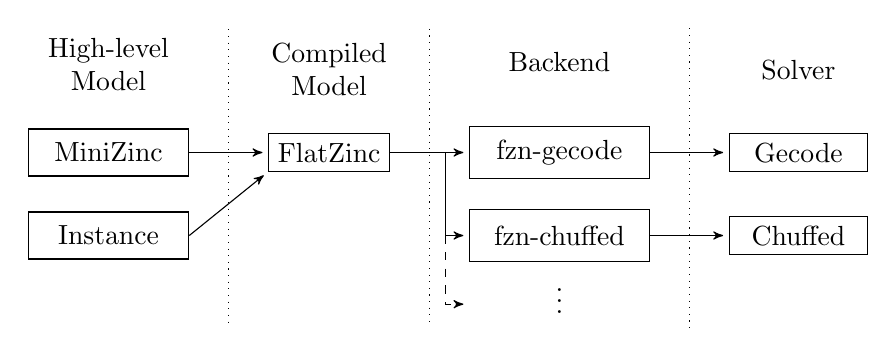
\begin{tikzpicture}[
  grunka/.style={rectangle,draw,align=center},
  grej/.style={align=center,rectangle},
  solver/.style={minimum width=50pt},
  backend/.style={minimum width=65pt,minimum height=19pt},
  model/.style={minimum width=58pt,minimum height=17pt},
  shorten >=2pt,
  >=stealth'
  ]
  \node [grunka,model] (MZN) at (0, 0) {MiniZinc};
  \node [grunka,model] (DZN) at ($(MZN.center) + (0, -30pt)$) {Instance};
  \node [grunka] (FZN) [right=of MZN] {FlatZinc};
  \node [grunka,backend] (BKN) [right=of FZN] {fzn-gecode};
  \node [grunka,solver] (SLV) [right=of BKN] {Gecode};
  \node [grunka,backend,anchor=west] (BKN2) at ($(BKN.west) + (0,-30pt)$) {fzn-chuffed};
  \node [grunka,solver] (SLV2) at (SLV|-BKN2) {Chuffed};
  \node (ELI) [below=5pt of BKN2] {$\vphantom{\int^0}\smash[t]{\vdots}$};

  \node [above=23pt of MZN,grej,anchor=center] {High-level \\ Model};
  \node [above=23pt of FZN,grej,anchor=center] {Compiled \\ Model};
  \node [above=23pt of BKN,grej,anchor=center] {Backend};
  \node [above=23pt of SLV,grej,anchor=center] {Solver};

  \draw[->] (MZN) edge (FZN)
            (FZN) edge (BKN)
            (BKN) edge (SLV)
            (BKN2) edge (SLV2);
  \draw[->] (DZN.east) -- (FZN.south west);
  \draw[->] ($(FZN.east)!0.7!(BKN.west)$) |- (BKN2);
  \draw[dashed,->] ($(FZN.east)!0.7!(BKN.west)$) |- (BKN2.west|-ELI);

  \verticalline{dotted}{($(MZN.east)!0.5!(FZN.west)$)};
  \verticalline{dotted}{($(FZN.east)!0.5!(BKN.west)$)};
  \verticalline{dotted}{($(BKN.east)!0.5!(SLV.west)$)};
\end{tikzpicture}%
\caption{How a MiniZinc model gets run by a solver to produce a result. The high-level model is compiled (flattened) into a low-level model which a backend and solver pair uses to find solutions.}%
\label{fig:minizinc}
\end{figure}


MiniZinc models are often divided into two parts: the model itself and instances. The
model is made generic in the sense that it models some problem, like TSP from
Section~\ref{sec:csp}, without exact values. The TSP model is in terms of $n$ cities, but
to be solved by a solver must $n$ have a concrete value, which instances (usually separate
files) provides. This distinction makes it very easy to run the same model with slightly
different values.

\subsubsection{Model Overview}\label{sec:mzn:syntax}
A MiniZinc model consists of (not limited to) decision variables, constraints, functions and solve statements.
Decision variables are values of various types like \mi{int}, \mi{bool} and \mi{float},
which the solver should find appropriate values for. What values are allowed
and how the variables should relate to each other is expressed in constraints. For
example, the following defines a decision variable \mi{x} of type \mi{int}, and a constraint which
constrains \mi{x} to have a value strictly greater than five.
\begin{mznnobreak}
var int: x;
constraint x > 5;
\end{mznnobreak}

\begin{sloppypar}
The solver needs to know what the goal is, and that is specified in a
\mi{solve}-statement. There are two modes: satisfaction and optimisation. Satisfaction
simply means to find values for all decision variables so that all constraints hold, and
optimisation means to find values to minimise or maximise some decision variable.
For example, adding \mi{solve minimize x;} to the example above would create a
model that tries to find the smallest integer value greater than five, which is
six. Adding \mi{solve satisfy;} would instead find \emph{any} integer greater than
five.
\end{sloppypar}

Variables that are fixed to a single given value are in MiniZinc called \emph{parameters}.
A parameter is declared with \mi{par}, or no keyword at all, instead of \mi{var}.
Parameters are useful since they can be seen as parameters for the whole model itself,
i.e.\@ what exact instance of a model that should be solved.
For example, the above example can be rewritten with a parameter as follows:
\begin{mznnobreak}
int: n = 5;
var int: x;
constraint x > n;
solve minimize x;
\end{mznnobreak}
Now we can easily change the value of \mi{n} to solve a slightly different problem.

This can be separated into a separate instance file by giving
% A powerful feature this allows for is to separate all (or some) parameters to another file
% called an instance file.
the model the declaration {\mi{int: n}} and the
instance file the assignment \mi{n = 5}. Multiple instance files can be created
for a single model, which makes it easy to change all parameters at once.

Arrays allows for a variable amount of variables. The example below shows an array \mi{xs}
consisting of five int-variables. A contained variable can be accessed separately with
some special syntax. For example, the first variable can be accessed with
\mi{xs[1]}.
\begin{mznnobreak}
array[1..5] of var int: xs;
constraint forall(i in 1..5)(xs[i] > 5);
\end{mznnobreak}
To access all variables in an array at once can the builtin function \mi{forall} be used.
The example above uses this to constrain all variables in the array to be strictly greater
than five, it is like writing: $\forall x \in xs : x > 5$.

The final feature that will be covered here is functions. Functions allows the modeller to
reuse the same code in multiple places. A function has a return value and zero or more
parameters (not instance parameters), all of which can have the same types as
variables. The declaration and usage of a function which takes a decision variable as
parameter and returns a decision variable is shown below:
\begin{mznnobreak}
function var int: a_name(var int: x) = <@\textit{<some expression>}@>;
constraint a_name(x) < n;
\end{mznnobreak}

Some functions are very special, and they are called \emph{global constraints}. A global
constraint is a function defined in the standard library for high-level modelling
abstractions. There is for example one called \mi{all_different} which constrains all
values in an array to all be different from each other. Many solvers implement
special inference algorithms for these, which basically means that they can reason a lot
better about them.

\subsection{Linters}\label{sec:bkg:linter}
% Lint is a program for doing static code analysis of C programs~\cite{lint}. The term
% \emph{linter} originates from this program and is nowadays a general term for any tool
% that performs static code analysis, except for things a compiler typically does, like
% syntax analysis and semantic analysis (type checking). Static in this context means that
% the analysis is done on the source code itself, without executing it.

A linter is a program for doing static analysis of source code, static meaning that the
analysis is done without running the program. A linter can look for bugs, enforce a
certain code style, find some kind of improvement, find error prone constructs, point out
special cases etc. Generally anything useful which the corresponding compiler isn't
already checking, which is syntax and semantic (type checking) analysis.
The term \emph{linter} originates from the program lint~\cite{lint}, a program for
analysing C programs. A compiler's main job is to convert the source code to something
else, usually machine code, and is probably aiming at doing so as fast as possible. This
is a reason as to why compilers aren't doing as many, or the same kinds of checks, as a
linter is doing~\cite{lint}.

Linters and other static analysis tools also exists for programming languages that are
interpreted, i.e.\@ languages that are run ``as is'' without compiling them first. Python
is an example of an dynamically typed (types determined at runtime) and interpreted
language. It is possible to put optional type information in a python program and have a
third-party program like mypy~\cite{mypy} do static type checking. MyPy does not
considered itself a linter as it performs type checking, something a compiler typically
does.

The checks a linter does are typically called \emph{rules}, and different linters have
different ways of specifying them. The JavaScript linter ESLint~\cite{ESLint} allows user
to create their own rules in separate JavaScript files, alongside the builtin ones. This
can be done dynamically because JavaScript is an interpreted language, so it can load new
code files during runtime a lot easier. A rule in ESLint
consists of a pattern match against the AST (see Section~\ref{sec:parsing}) and a function
which will do additional checks to see whether it is a match or not and if something
should be reported to the user. The rules in this project are structured in the same
manner, except that the part that pattern matches isn't as powerful. The one in ESLint can
find arbitrary sub-trees while the one in this project can only find paths (sub-trees that
are a line) in the AST.

The programming language Rust has a linter called Clippy~\cite{Clippy}. Rust is an
compiled language and rules to Clippy are specified as Rust source code. This means that
any new custom lint rule has to recompile the whole linter to be used, similar to this
project. Clippy rules are specified in a similar way to ESLint, with the difference on how
the AST is traversed. Each Clippy rule has special functions that are called on various
items in the language, like function declarations and struct declarations. Each of these
special functions determined if there is anything relevant to report to the user for that
construct.

There are many terms for when a rule finds a match for something it wants to report on.
\emph{Hits}, \emph{matches}, \emph{finds}, \emph{gets triggered} and \emph{reports} are
some that will be used in this report.

Rules in linters are usually divided into several groups so they can be disabled or
enabled more easily. An example of this could be to disable rules about white space and
indentation.
They also usually have unique identification numbers or names so they can be individually
disabled if desired.

\paragraph{Example}
The tool ShellCheck~\cite{shellcheck} is a linter for shell scripts, e.g.\@ bash. The
construct \texttt{"\$@"} expands to all arguments passed to the current script, useful if
all arguments should be processed to determine the script's behaviour. The quotes are
really important, since the expression without them will perform additional word splitting
on the arguments (and something called ``globbing''), which is not desired in the majority
of cases. Consider a script called with the arguments ``-f'' and ``my cool model.mzn''.
The expression \texttt{"\$@"} will expand in to the same arguments, i.e.\@ ``-f'' and ``my
cool model.mzn''. But without quotes, i.e.\@ \texttt{\$@}, it will instead expand to ``-f'',
``my'', ``cool'' and ``model.mzn'', they have been word split! This behaviour can be
frustrating to debug, so that is why the lint rule
called ``SC2068'' in ShellCheck does exactly this analysis.

\subsection{Parsing and Abstract Syntax Trees}\label{sec:parsing}
To be able to process source code, or models in text format, it is common to parse them
into some kind of data structure. There are many tools available called ``parser
generators'', which are programs that takes some kind of formal description of the
language to be parsed and generates source code in some programming language for a parser.
MiniZinc uses a parser generator called Bison~\cite{flexbison}, which is a generator that
can generate C++ code, the same language that MiniZinc is written in.

The output of a parser is often an Abstract Syntax Tree (AST), an example of which is
given in Figure~\ref{fig:bkg:ast}. The AST is representing the formal structure of the
source code as nodes with other nodes children. A function in C++ could for example be
represented as a node with a child for every statement in that function. Each statement is
itself a tree encoding whatever that statement is. The information
about the arguments and the return type could be stored in the node itself or as yet more
children, there are many ways to construct an AST.

An AST is abstract in the sense that it doesn't encode everything in the original code.
Things like parentheses in mathematical expression are often implicitly encoded by the
position each operator has in the tree, an example of this is shown in
Figure~\ref{fig:bkg:ast}. Those trees are evaluated bottom up, and each node's value is
its operation applied to the results of its child nodes. Nodes high up in the tree are
therefore evaluated \emph{after} its child nodes, which means that sub-expressions that
should be evaluated first, like expressions in parenthesis, are placed further down in the
tree.

\begin{tikzpicture}[AST, eval/.style={red, font=\footnotesize}]
  \node (l) at (0, 0) {*}
    child {node {0}}
    child {node {+}
      child {node {2}}
      child {node {$f$}
        child {node {3}}}};

  \node [eval, above right=-6pt and 0pt of l-2-2-1] {3};
  \node [eval, above right=-6pt and 0pt of l-2-2] {3};
  \node [eval, above right=-6pt and 0pt of l-2-1] {2};
  \node [eval, above right=-6pt and 0pt of l-2] {5};
  \node [eval, above right=-6pt and 0pt of l-1] {0};
  \node [eval, above right=-6pt and 0pt of l] {0};

  \node (r) at (6, 0) {+}
    child {node {*}
      child {node {0}}
      child {node {2}}}
    child {node {$f$}
      child {node {3}}};

  \node [eval, above right=-6pt and 0pt of r-2-1] {3};
  \node [eval, above right=-6pt and 0pt of r-2] {3};
  \node [eval, above right=-6pt and 0pt of r-1-1] {0};
  \node [eval, above right=-6pt and 0pt of r-1-2] {2};
  \node [eval, above right=-6pt and 0pt of r-1] {0};
  \node [eval, above right=-6pt and 0pt of r] {3};
\end{tikzpicture}


\section{Implementation}\label{sec:impl}
This project is implemented using C++~\cite{cpp}, a compiled programming language with
performance as a main design goal. The same MiniZinc parser as the MiniZinc project is
using was used in this project as well. This project will only analyse
the Abstract Syntax Tree (AST) given from the parser, so it is unnecessary to write a new
parser which would do the exact same thing. Using the same AST would also make it possible
to reuse other utilities present in the MiniZinc compiler, such as the type checker and
pretty printer (converting the AST back to nicely formatted code). It is also easier to
maintain one parser as opposed to two. As the MiniZinc
compiler is written in C++ was creating this project in the same language a natural
choice. C++ comes in several different standards, and C++17 was the one used for this
project as that was the latest one all major compilers fully supported at the time this
project started. The MiniZinc version is 2.5.5 as, again, that was the latest version when
this project started.

An overview of how the program itself is structured is explained in
Section~\ref{sec:impl:structure}. The AST searcher will be explained in detail in
Section~\ref{sec:searcher}.

\subsection{Overall Structure}\label{sec:impl:structure}
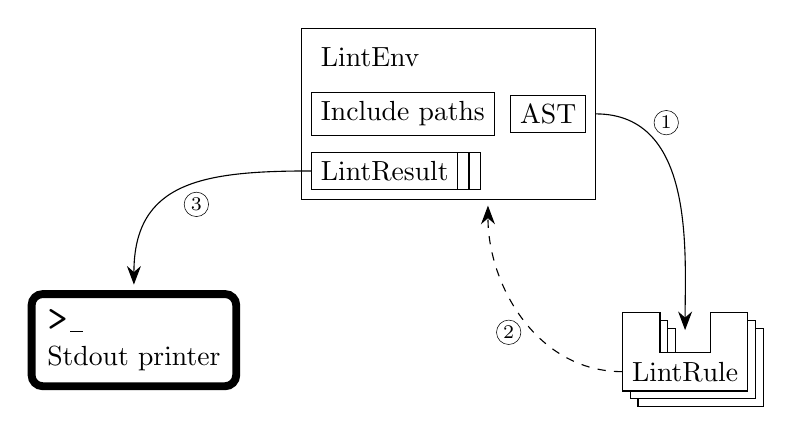
\begin{tikzpicture}[
  blackrekt/.style={draw, rectangle},
  number/.style={auto,draw,circle,solid,inner sep=1pt,outer sep=3pt, node font=\scriptsize, very thin},
]
  \node (LE) at (0, 0) {\cpp{LintEnv}};
  \node (IP) [blackrekt, below=0.2 of LE.south west, anchor=north west] {Include paths};
  \node (AST) [blackrekt, right=0.2 of IP] {AST};
  \node (RES) [double copy shadow={shadow xshift=4pt, shadow yshift=0}, fill=white, blackrekt, below=0.2 of IP.south west, anchor=north west] {\cpp{LintResult}};
  \node (BOX) [fit=(LE) (IP) (AST) (RES), blackrekt] {};

  \newcommand{\lintrule}[2]{
    \node (#1) at #2 {\cpp{LintRule}};
    \draw[fill=white] (#1.north west) +(0, 0.5) -| ($(#1.north west)!0.3!(#1.north east)$)
    -- ($(#1.north west)!0.7!(#1.north east)$) |- ($(#1.north east) + (0, 0.5)$)
    -- (#1.south east) -- (#1.south west) -- cycle;
  }
  \foreach \y in {-4.2, -4.1, -4} \lintrule{LR1}{(-\y, \y)};
  \node (PR1) at (4, -4) {\cpp{LintRule}};
  \draw[big arrow, shorten >=8pt] (BOX) edge[out=0, in=90] node [number, near start] {1} (LR1);
  \draw[big arrow, dashed] (LR1) edge[out=180,
  in=-90] node [number] {2} ($(BOX.south) + (0.5, 0)$);

  \node (PRT) [rectangle, align=left, draw=black, line width=1mm, rounded corners, inner sep=2mm] at (-3, -3.6) {\texttt{\textbf{\Large >\_}} \\ Stdout printer};
  \draw [big arrow] (RES) edge[in=90,out=180,looseness=1.3] node [number] {3} (PRT);

\end{tikzpicture}%


The overall structure is illustrated in Figure~\ref{fig:overview} and everything following
here will be illustrated in that figure.
The most important component of this linter is a base class called \cpp{LintRule}. Each
rule described in Section~\ref{sec:rules} is its own class that inherits from
\cpp{LintRule}. Each rule consists of a unique id, a category, %TODO: elr?
a name and finally a method which accepts a model and returns the results, if any. This
model argument is an object of the class \cpp{Model}, i.e.\@ the AST from the parser in
the MiniZinc project. They will be referred to as ``AST'' to avoid confusion with model
files. The id and category are used for filtering which rules to use, and the name is used
for printing purposes. Each rule performs its analysis generally by first searching in the
AST for a relevant construct, which for example could be a variable used inside an
\mi{if}-statement. They do this search by using a custom searcher described in
Section~\ref{sec:searcher}. When a construct is found are multiple checks or other
processing done to figure out whether this construct should be reported to the user or not.

\begin{sloppypar}
The rules don't take the AST directly, they take it wrapped in a class called
\cpp{LintEnv}. This class contains a lot of helper functions that each rule interacts with
directly. \cpp{LintEnv} contains, aside from the AST, a list with file paths to search for
libraries in, i.e.\@ include paths. MiniZinc comes with a standard library that many
common MiniZinc functions are defined in (global constraints), and include paths help the linter to find them.
\cpp{LintEnv} also contain all results and methods to create new ones. The final thing
this class does is caching the results from common searches performed by the AST searcher.
One such search is finding all user-defined
variables, both top-level and defined in \mi{let}-statements.
\end{sloppypar}

Each result is recorded in a class called \cpp{LintResult}. These hold the relevant data
for a result like what rule it came from, the file position (line and column) for where it
matched, an explanatory message, a recommended rewrite of the model etc. These results are
then given to some function which will present them to the user. That can be a simple
print to standard output in a human-readable form, or converted to the JSON-format and
given to an IDE, or anything else.

These are all of the relevant components for a high-level overview of this linter. A
typical execution for this linter in terms of these components is as follows:
\begin{enumerate}
  \item Gather options and model files from the arguments of the process
  \item Parse to file into a \cpp{Model} class (AST), abort on errors
  \item Type check the AST, abort on errors
  \item Create \cpp{LintEnv}
  \item Iterate through all \cpp{LintRule} and run them
  \item Give the list of all \cpp{LintResult} to a function which will output them to, e.g.\@
  standard out
\end{enumerate}

\subsection{Abstract Syntax Tree Searcher}\label{sec:searcher}
This project uses a custom made algorithm for finding relevant positions of interest in
MiniZinc Abstract Syntax Trees (ASTs). Many rules require more complex searches than
simple matching of single nodes in the AST, e.g.\@ ``find x=3 anywhere inside constraints
except for in the else clause of if-statements'' over ``find all if-statements''. Creating
a searcher for this made the implementation of all rules a lot simpler. An alternative
would be to use what the MiniZinc project already is using for processing the AST, namely
visitors~\cite{DesignPatterns94}. It would be easy to find single nodes of interest using
visitors, but it would be a lot more verbose to find anything more complicated than that.

\subsubsection{MiniZinc Abstract Syntax Tree}
\ifshowastnumbers\newcounter{asdasd}\fi
\begin{tikzpicture}[
label distance=-10pt,
every label/.style={blue},
lbl/.style={label=160:{\ifshowastnumbers\stepcounter{asdasd}\arabic{asdasd}\fi}}
]
  \node at (0, 0) {\mi{constraint}} [sibling distance=60pt]
  child {node[lbl] {\cpp{BinOp} =}
    child {node[lbl] {\cpp{BinOp} +}
      child {node[lbl] (X) {\cpp{Id} ``x''}}
      child {node[lbl] {\cpp{IntLit} 42}}
    }
    child {node[lbl] {\cpp{Id} ``y''}}
  };

  \node (VX) at (6.5, 0) {\mi{var int: x}} [level 2/.style={sibling distance=140pt}, level 3/.style={sibling distance=65pt}]
  child {node[lbl] {\cpp{BinOp} +}
    child {node[lbl] {\cpp{BinOp} +}
      child {node[lbl] {\cpp{IntLit} 1}}
      child {node[lbl] {\cpp{IntLit} 1}}
    }
    child {node[label=177:{\ifshowastnumbers\stepcounter{asdasd}\arabic{asdasd}\fi}] {\cpp{BinOp} +}
      child {node[lbl] {\cpp{IntLit} 1}}
      child {node[lbl] {\cpp{IntLit} 1}}
    }
  };

  \draw[-{Straight Barb[scale=1.3]},dashed] plot [smooth] coordinates {(X.south) ($(X.south) + (3, -0.3)$) ($(VX.west) + (-1.2, -0.5)$) (VX.west)};
\end{tikzpicture}


The output of the MiniZinc parser is an object of the class \mi{Model}. It is not strictly
an abstract syntax \emph{tree}, but more like a collection of abstract syntax
\emph{graphs}. An illustration of this is show in Figure~\ref{fig:ast:searcher}.
\mi{Model} contains a list of all top-level items in a model, like constraints, variable
declarations and functions. Each of those contain one or more \emph{expressions}, which
basically are things that can be evaluated to some value, e.g.\@ \mi{1+1} which can be
evaluated to \mi{2}. Each expression is not strictly a tree either since for example
\cpp{Id}-nodes, which represent an identifier like ``x'', has a pointer to the variable
declaration it is referring to. The searcher explained here will actually search in these
expressions individually, but the whole model will be referred to as one AST for
simplicity.

Each expression saves where it came from, they save: the filename, beginning line, end
line, beginning column and end column. If an expression didn't come directly from a file,
but was auto generated, it is marked as ``introduced'' instead.

\subsubsection{Finding Paths}\label{sec:paths}
The searcher works by finding paths in the AST, i.e.\@ a sequence of nodes
$n_1, n_2 \dots n_k$ $k \in \elnaturale^+$ where $n_m$ is a direct child of $n_{m-1}$ for
all $m \in \{2,\dots,k\}$. A target path, or path to be searched for, is given as a
non-empty sequence of targets $T_{R,N}$. Where $N$ is what kind of AST node to match
against and $R \in \{U,D\}$ specifies how a node matched by a target relates to the node
matched by the previous target in the sequence. The value $D$ (``direct'') means that the
node matched should be a direct child of the previous match, and $U$ (``under'') means
that the node can be anywhere under the previous match. If $T_{R,N}$ is the first target
in the sequence is $R$ not relating to the previous match, but to an implicit dummy node
that only has the root as child.
A value of $D$ would therefore mean that the match has to be the root of the tree and $U$ would mean
that it can occur anywhere.

For example, the sequence $\langle T_{D,=} \; T_{U,+} \rangle$ will match a \cpp{BinOp}~=
at the root of the AST, and then match a \cpp{BinOp}~+ anywhere on either the left-hand
side or right-hand side of the equal-node. Taking the left tree in
Figure~\ref{fig:ast:searcher} as an example, this sequence will give the path
$\langle 1,2 \rangle$ as a match.

Another example is the target sequence
$\langle T_{U,+} \; T_{U,\text{\mi{IntLit}}} \rangle$, this will match a plus-node
anywhere that has a integer literal anywhere under it. The left tree in
Figure~\ref{fig:ast:searcher} has one path matching this, namely $\langle 2, 4 \rangle$.
The right tree on the same Figure has a couple of more matches, namely:
$\langle 6, 8 \rangle$, $\langle 6, 9 \rangle$, $\langle 6, 11 \rangle$,
$\langle 6, 12 \rangle$, $\langle 7, 8 \rangle$, $\langle 7, 9 \rangle$,
$\langle 10, 11 \rangle$, and $\langle 10, 12 \rangle$.

\subsubsection{Algorithm}\label{sec:algo}
This path matching algorithm is implemented as a backtracking algorithm. It will do a
Depth First Search (DFS) to iterate over all paths in the AST. If the algorithm at some
points deduces that the current path can't possibly produce a full match for a sequence of
targets, it will stop searching that path and backtrack to an earlier point and try again.

The algorithm is given an
AST of $m \in \elnaturale^+$ nodes, and a sequence $S_1, S_2, \dots, S_k$ of $k \in \elnaturale^+$ targets as
explained in Section~\ref{sec:paths}. It maintains a stack $D$ for a DFS of the
AST, and another stack $P$ which contains the current path the DFS is on. Nodes get pushed
to $P$ as they are discovered, but it must also know when to pop them of $P$. For this,
the algorithm
has to know when a particular node's children are done searching. Lets say that the DFS
popped a new node $n$ from $D$, it will push $n$ to $P$ to update the current path, but it will
also push it back to $D$, as a marker, followed by all children of $n$. Now, if at any point later in
the search $n$ gets popped again from $D$ and the top element of $P$ also is $n$, the DFS
algorithm now knows that all sub-nodes of $n$ have been processed and that it is now okay to pop $P$.

Some nodes in $P$ will be matched nodes from $S_n$, and some will be ``nodes on the way''
when ``under'' is used. Only the matched nodes are of interest, so yet another stack $H$
will keep track of the same path as $P$ but only store nodes matched directly from all $S_n$.
$H$ is therefore a sub-stack of $P$, and
$H$ will have a maximum size of $k$ while $P$ will have a maximum size equal to
the height of the AST.

A function $U$
will determine whether a target $S_n$ is ``under'' (see Section~\ref{sec:paths}). $D$ is
initialised with the root node of the AST and $P = H = \emptyset$. $1 \leq x \leq k+1$ will be the index of
the next \emph{unmatched} target to find. If $x = k+1$ are all targets are matched.
% The pseudo code is shown in Figure~\ref{fig:algo:code}.
The pseudo code is as follows:

% \begin{figure}
\begin{enumerate}[noitemsep]
  \item\label{alg:beg} abort if $D = \emptyset$
  \item $d = \mathtt{pop}(D)$
  \item if $d = \mathtt{top}(P)$, a marker was popped
    \begin{enumerate}
      \item $\mathtt{pop}(P)$, $d$ is no longer on the current path
      \item if $d = \mathtt{top}(H)$
      \begin{enumerate}
        \item $\mathtt{pop}(H)$ and $x \gets x-1$
        \item if $U(S_x)$, push $d$ to $P$ and $D$, and also all children of $d$ to $D$.
        This step forces $d$ to be unmatched to allow other nodes under $d$ to
        be matched against $S_x$.
      \end{enumerate}
      \item go to~\ref{alg:beg}
    \end{enumerate}
  \item if $S_x$ matches $d$
    \begin{description}
      \item[true] $x \gets x+1$, push $d$ to $H$ as it is an match
      \item[false] go back to \ref{alg:beg} if $U(S_x) = \top$. $S_x$ had to match
      directly after $S_{x-1}$ (the previous), but it didn't
    \end{description}
  \item push $d$ to $P$, it is now part of the current path. Also push $d$ to $D$ as a marker
  \item if all $S$ have matched ($x > k$), $P$ contains a whole match. Go to~\ref{alg:beg}
  \item push all children of $d$ to $D$
  \item go to~\ref{alg:beg}
\end{enumerate}
% \caption{}%
% \label{fig:algo:code}
% \end{figure}

\paragraph{Complexity}
The worst case run-time depends mostly on how many ``under'' there are and what shape the
tree is in. The worst case is when all targets are ``under'', i.e.\@ $\forall_{1 \leq x
  \leq k} : U(S_x)$. Consider that the AST is a straight line that is $m$
nodes long and that there are $k$ targets to match. If all $S_n$ match on every node will the
searcher iterate over all $\binom{m}{k}$ matches. An upper bound can be found from the
definition:
\begin{equation*}
  \binom{m}{k} = \frac{m!}{k! (m-k)!} = \frac{m}{k} \cdot \frac{m-1}{k-1} \dots \frac{m -
    (k-1)}{1} \leq \frac{m^k}{k!}
\end{equation*}%
%TODO: todo
The worst-case complexity is then $\Oh{{m^k}/{k!}}$\todo{can k! disappear if m>k? (which
  it is) Or it maybe doesn't matter}, at least for when the AST is a line. If the AST was instead a
tree would there not be as many matches since not all $\binom{m}{k}$ choices of nodes is
on a path from the root, so it would not be as bad.

This scary worst-case complexity is
not such a huge problem as only \emph{one} instance of this searcher in the final implementation
had two ``under'' targets, all other 28 only had one or none at all. This analysis also
assumed that each target matched everywhere, but that is far from the case (most of the
time) as each target matches a \emph{single} type of node, and there are many different
kinds. The searcher will therefore most often than not stop early in the tree, so most of
all $\binom{m}{k}$ cases are not even checked. More is discussed in Section~\ref{sec:resultat},
\nameref{sec:resultat}.

\subsubsection{Filter Out the Standard Library}\label{sec:filter:stdlib}
Different kinds of filtering is performed by the searcher. Each target $T_{R,N}$
(explained in Section~\ref{sec:paths}) can have a function $F(n,c)$ which is used to
determine whether child $c$ of $n$ should be searched or not. This can be used to, for
example, make sure only the left-hand side of a binary operator is searched upon. In
general it makes a search more specific and fine-tuned.

Only considering user-defined variables, functions, constraints etc.\@ is another kind of
filtering this searcher does. Given an include path to the standard library, the searcher
will not search in functions and variables whose origin filename is somewhere inside the
include path. It will also ignore those whose location is introduced.

\section{Linting rules}\label{sec:rules}
% TODO: todo
\todo{show how a rule is implemented in terms of the searcher maybe}
In this section will all currently implemented rules be explained, both why they are good
and in some cases also how they are implemented. Some of these rules comes from a
startup meeting with me, the reviewer, the supervisor, some of MiniZinc's creators and others
with a lot of experience with MiniZinc and solvers. Some rules comes from a course on
combinatorial optimisation which the supervisor is teaching.

The rules vary in complexity and preciseness. Some rules build graphs and provide very
confident answers, while others simply mark decision variables in places where it is
\emph{generally} bad to have them. Some rules are more of an heads up than something that
should be fixed.

Further reading for more in-depth explanations are available in the MiniZinc
Handbook~\cite{mznbook}. Links to sections in that documentation will be provided where
relevant. The MiniZinc version and exact location can for the most part be parsed from
these links, useful in case they change in the future.

\subsection{General Design Decisions}\label{sec:rule:design}
One design decision was to not rely on instances, i.e.\@ the rules should work even if not
all parameters have values. The rationale is that all rules should be valid for all
instances of a given model. This limits the ability of some rules, notably \ruleref{constvar}, as they can't always
draw all types of conclusions. An example of this is the question whether a \mi{forall}
accesses all values in an array or not. The following silly model demonstrates a case
where it is impossible to know:

\begin{mznnobreak}
int: N; int: K;
array[1..N] of var int: a;
constraint forall(i in 1..K)(a[i] = <@\dots@>);
\end{mznnobreak}

The \mi{forall} accesses all values if \mi{N} is equal to \mi{K}, but that is not
guaranteed to be the case, so the linter will assume that the \mi{forall} does not access
all values. If the \mi{forall} used the exact same set as the array (\mi{1..N}), then the
linter could know that all values were accessed. Some rules will provide results anyway,
even if they depend on parameters, but the linter will warn the user in those cases so an
accidental rewrite that breaks the model in the future is not made.

\subsection{Arrays Start at One}\label{sec:rule:arrayatone}
Arrays that start at 1 are more efficient and easier to understand.
\begin{mznnobreak}
array[1..4] of var int: good;
array[5..9] of var int: bad;
\end{mznnobreak}
Flattened arrays always start at 1, so each array access to an array which do not start at
1 has to first be translated. If the access is from a decision variable, i.e.\@ the \mi{i} in \mi{a[i]} is
\mi{var} is an additional variable introduced that translates \mi{i} to an index that
starts at one. More details can be found under ``Arrays'' in ``flattening'' in the
documentation\footnote{\url{https://www.minizinc.org/doc-2.5.5/en/flattening.html\#arrays}}


\subsection{Compactable If-statement}\label{sec:rule:compactif}
If-statements on the form:

\begin{mznnobreak}
var bool: b; var int: z; var int: y;
constraint z = if b then y else 0 endif;
constraint z = if b then 0 else y endif;
\end{mznnobreak}

can be rewritten to more compact versions using implicit bool conversions (false converts
to 0 and true converts to 1):

\begin{mznnobreak}
constraint z = b*y;
constraint z = (not b)*y;
\end{mznnobreak}

These rewrites tend to be faster and produce fewer FlatZinc constraints.

\subsection{Constant Variable}\label{sec:rule:constvar}
A decision variable or an array of decision variables that are all assigned to non-variables should not be
marked with \mi{var} as their values are constant. It marks the intent of the value more
clearly, and makes it easier for the compiler. Some examples where the keyword \mi{var}
should be omitted or replaced with \mi{par}:

\begin{mznnobreak}
var int: x = 2;
array[int] of var int: a = [1, 2, 3];
\end{mznnobreak}

This rule also checks if a \mi{var} is constrained to a \mi{par}-value:

\begin{mznnobreak}
var int: x;
constraint x = 2;
\end{mznnobreak}

This rule also checks if all values in an array is constrained to \mi{par}-values for
simple cases, some limitations explained in Section~\ref{sec:rule:design}.

\begin{mznnobreak}
array[1..5] of var int: a;
constraint forall(i in 1..5)(a[i] = 1);
\end{mznnobreak}

\subsection{Effective 0..1 Variables}\label{sec:rule:zeroone}
Some expressions can be rewritten to a often better performing expression if the domains in
question happens to be $\{0,1\}$. For example, if there are two variables declared as
\mi{var 0..1: a} and \mi{var 0..1: b} can the expression \mi{a=1 -> b=1} be rewritten
to the equivalent \mi{a<=b}. In the same way can \mi{a=0 -> b=0} be rewritten to \mi{a>=b}.
Finally is this rule also suggesting to rewrite \mi{sum(i in S)(a[i] = 1)} to the
equivalent \mi{sum(a)} if \mi{array[S] of var 0..1: a}. This one is especially good
as the first variant is doing implicit conversions between bools and integers
(\mi{bool2int}) while the rewrite isn't.

The expressions on either side (\mi{a} and \mi{b}) can be arbitrarily complex, as long as
their domains can be calculated. If either depends on the current instance is a warning
issued, as discussed in Section~\ref{sec:rule:design}. If that parameter is changed might
these rewrites not be valid anymore, so the modeller should think twice before rewriting.

\subsection{Element Predicate}\label{sec:rule:element}
The predicate \mi{element} is a function which takes an index (\emph{i}), an array
(\emph{a}) and a value (\emph{v}) and returns true if the element at \emph{i} in the array
\emph{a} is equal to \emph{v}. \mi{element(i, a, v)} is a more verbose way of writing
\mi{a[i] = v}, \mi{element} is even defined as that. The array
access syntax should be used instead to make the model more easy to read.

\subsection{Global Constraint Reified}\label{sec:rule:reifiedglobal}
A global constraint called in a reified context \emph{can} be slow and inefficient,
and this rule will mark all those occasions. Being reified means that the result of the global
constraint is bound to a boolean variable, i.e.\@
\begin{mznnobreak}
var bool: x = all_different(a);
\end{mznnobreak}
Reification happens when the global constraint is called in a context which is not $\land$.
For example, this global constraint will be reified:
\begin{mznnobreak}
constraint b \/ all_different(a);
\end{mznnobreak}
and the following is always okay:
\begin{mznnobreak}
constraint all_different(a);
constraint all_different(b) /\ all_different(c);
\end{mznnobreak}
The official MiniZinc documentation talks more about this under ``Reified and half-reified
predicates''\footnote{\url{https://www.minizinc.org/doc-2.5.5/en/fzn-spec.html\#reified-and-half-reified-predicates}}
and under ``Reification''\footnote{\url{https://www.minizinc.org/doc-2.5.5/en/flattening.html\#reification}}.

The linter will consider all functions from the standard library as global constraints,
except for those that don't have to be included, like \mi{forall}.

\subsection{Global Variables in Functions}\label{sec:rule:blobalfun}
Using variable from the global scope in functions is usually confusing as the whole model
(or at least everything required to understand the purpose of the global variable in
question) has to be read and understood to understand the function. It is also not
immediately as clear as to what variables a function is constraining and accessing. This rule
suggest to take all those variables as arguments to the function instead.

\begin{mznnobreak}
var int: g;
function int: f() = g+1;
constraint f() = 2;
\end{mznnobreak}
is suggested to be rewritten to:
\begin{mznnobreak}
var int: g;
function int: f(var int: x) = x+1;
constraint f(g) = 2;
\end{mznnobreak}

Only decision variables are marked as parameter values can only be read from, and are like
parameters to the whole model itself, so they have to be understood anyway.

\subsection{No Domain on Variables}\label{sec:rule:nodomain}
Variables can specify a domain which the variable can take values from. It is always
recommended to specify a tight domain for decision variables as not specifying one at all
makes the domain \emph{very} large and makes the solving unnecessarily slow.
\begin{mznnobreak}
var int: bad;
var 0..5: good;
\end{mznnobreak}
If the variable is assigned a value, even another variable, makes it fine to omit the domain
as it can be referred from the assigned value. Constraining them is also fine.
\begin{mznnobreak}
var 10..20: good;
var int: also_good = good;
var int: also_good2;
constraint also_good2 = good;
\end{mznnobreak}
This rule marks unassigned decision variables that have no explicit domain given.
More can be read in ``Bounds analysis''\footnote{\url{https://www.minizinc.org/doc-2.5.5/en/efficient.html\#variable-bounds}}.

\subsection{Non-functionally Defined Variables not in Search Hint}\label{sec:rule:nonfuncdef}
%TODO: todo!
Stay tuned!

\subsection{Operators on Variables}\label{sec:rule:opvar}
Some operators like \mi{div} and \mi{pow} are expensive to do on variables. Pre-computing
these and store them in a table (tabling) is recommended if feasible as the expansive calculations are
done once, before the solving has started.

Operators like \mi{\\/} and \mi{->} on variables can also be expensive as they introduce
more branching in solvers.\todo{is this even true? Something should be referenced here} %TODO: verify

This rule blindly recommends to avoid using these operators on variables.

\subsection{Symmetry Breaking Missing}\label{sec:rule:symbreak}
Some global constraints like \mi{value_precede_chain} are almost only used to break
symmetries in models. Breaking symmetries is important since it speeds up solving by
reducing the amount of possible solutions that has to be explored. Constraints whose
purpose is break symmetries should be marked as such:
\begin{mznnobreak}
constraint symmetry_breaking_constraint(<@\dots@>);
\end{mznnobreak}
Some solving techniques, like local search, are negatively impacted
by symmetry breakers, so solvers which use technologies like that ignore all marked
symmetry breaking constraints. So this rule blindly marks global constraints which are
normally used for breaking symmetries. More general theory about this can be found in
``Effective modelling practices''\footnote{\url{https://www.minizinc.org/doc-2.5.5/en/efficient.html\#symmetry}}.

\subsection{Unused Variables and Functions}\label{sec:rule:unused}
This rule wants to remove variables and functions which are not used anywhere.
Used in this case means to be mentioned inside constraints, the solve statement or other
functions and variables which are also in use. The output-statement is an exception and
don't contribute to the usage of variables and functions. The rationale is that only being
mentioned in the output statement doesn't contribute to the model, i.e.\@ the amount of
solutions don't change.

To calculate whether a variable or function is unused is a dependency graph first
constructed. This directed graph will keep track of which variables and functions use
which other variables and functions. The graph for the following example is shown in
Figure~\ref{fig:unused:graph}.

\begin{mznnobreak}
int: K; int: N;
int: M = let {int: J = 5} in J+N;
var 0..K: x;
function var int: f() = x+N;
solve minimize f();
\end{mznnobreak}

\begin{figure}[ht]
\centering
\smallskip%
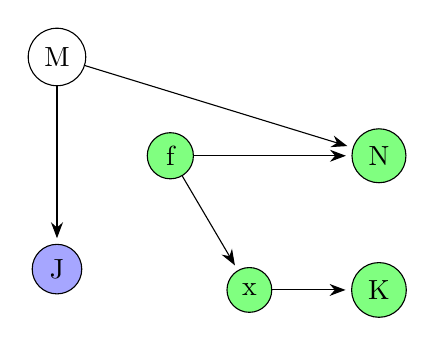
\begin{tikzpicture}[
  every node/.style={draw, circle},
  -{Stealth[scale=1.2]},
  shorten >=2pt,
  used/.style={fill=green!50!white},
  contained/.style={fill=blue!35!white},
  ]
  \node (K) [used] at (0, 0) {\mi{K}};
  \node (x) [left=of K, used] {\mi{x}};
  \node (N) [above=of K, used] {\mi{N}};
  \node (f) [left=2 of N, used] {\mi{f}};
  \node (J) [below left=of f, contained] {\mi{J}};
  \node (M) [above=2 of J] {\mi{M}};

  \draw (x) edge (K)
        (f) edge (x)
        (f) edge (N)
        (M) edge (J)
        (M) edge (N);
\end{tikzpicture}%
\smallskip%
\caption{A dependency graph of an example model. An edge from a node to another means that
  the first node is directly depending on the other. For example is \mi{M} using \mi{N}.
  The green filled in nodes (\mi{f}, \mi{N}, \mi{x} and \mi{K}) are in use, and the blue
  filled node (\mi{J}) is ignored as it is contained inside of \mi{M}.}%
\label{fig:unused:graph}
\end{figure}


After the graph has been constructed are all constraints and solve-statements checked for
mentions of any variables and functions, and for each one is it and all of its
dependants marked as used. In this example is \mi{f} used in the solve-statement, so
\mi{f}, \mi{N}, \mi{x} and \mi{K} are thus marked as used. In this case are there no
constraints, so \mi{J} and \mi{M} are left as unused.

Reporting both \mi{J} and \mi{M} in this case might seem excessive since \mi{J} is
``inside'' of \mi{M}, so if \mi{M} is unused is it obvious that \mi{J} also is unused.
This is even more of a problem with unused functions, as each argument and variable inside
of it also will be individually reported. To solve this and only report on the outermost
variable or function is another graph constructed, a containment graph. In this case is
only \mi{J} inside another variable or function, namely \mi{M}. This containment graph is
inspected after all variables and functions have been deemed used or unused, and each
unused variable or function which is inside something else which also is unused gets
ignored. So in this case is only \mi{M} reported to the user as unused.

\subsection{Variables in Generators}\label{sec:rule:vargen}
This rule blindly reports on decision variables used in generators. This is generally
always bad and should be avoided.

\begin{mznnobreak}
var 1..5: x;
constraint forall(i in 1..x)(<@\dots@>);
\end{mznnobreak}

A \mi{forall} is unrolled into several separate constraints when flattened, one for each
value of \mi{i} in this case. But when the exact amount of constraints is unknown must the
flattener do more complicated things. More about unrolling can be read in ``Unrolling
Expressions''\footnote{\url{https://www.minizinc.org/doc-2.5.5/en/flattening.html\#unrolling-expressions}}
and ``Hidden Option Types''\footnote{\label{foot:hidden:opt}\url{https://www.minizinc.org/doc-2.5.5/en/optiontypes.html\#hidden-option-types}}.

\subsection{Variables in If and Where}\label{sec:rule:varif}
This rule will blindly mark decision variables used in \mi{where} clauses and the deciding
part on \mi{if}-statements, as that can slow down solving. Examples of this are:

\begin{mznnobreak}
var bool: b;
constraint if b then <@\dots@> else <@\dots@> endif;
\end{mznnobreak}
\begin{mznnobreak}
array[<@\dots@>] of var int: a;
constraint forall(i in <@\dots@> where a[i] > 5)(<@\dots@>);
\end{mznnobreak}

These will make the models more complex and should preferably be avoided if possible.
More about the \mi{where} case can be read about under ``Hidden Option
Types''\footnote{\label{foot:hidden:opt}\url{https://www.minizinc.org/doc-2.5.5/en/optiontypes.html\#hidden-option-types}}.

\section{Results and Discussion}\label{sec:resultat}
The linter was run one all models in the MiniZinc Benchmarks~\cite{mznbench}, which is a
big repository of models and instances where most (or all?) comes from earlier MiniZinc
challenges~\cite{MZN:Challenge}, a competition for solvers.
There were many rule hits throughout all models here, which isn't surprising as most rules
are general recommendations, so most of these hits are probably false positives. It
doesn't mean that they are useless though, as they will make the modeller think twice
about e.g.\@ dividing a decision variable.

\subsection{Performance}
It took in total around 23 %TODO: minizinc benchmark
seconds to lint all 299 model files. It took in total around 13 seconds when only running
the parser and type checker. That means that around $(23-13)/299 = 0.033$ seconds
(\SI{33}{\milli\second}) was spent on checking all rules on average (on my computer at least). %TODO: inte my computer

The exponential
worst-case complexity presented in Section~\ref{sec:algo} doesn't seem to cause too much
of an issue. Beyond what is said there about not being as bad as it seems is it also the
case that each top-level expression is relatively small, i.e.\@ a few number
of AST nodes, at least in most benchmark models (there are some gigantic ones that seem
auto generated). The algorithm can probably be improved to something with better
worst-case. The problem is essentially to match a regular expression over many strings
with common prefixes, except that the characters are node ids and the strings are paths
from the root of an AST.

%TODO: metod som förklarar hur det evalueras
%TODO: ett exempel på model som blir bättre
\subsection{Reflection on Benchmark Results}%TODO: bättre titel
All rules were triggered at least twice when run on all models in the MiniZinc benchmark,
except for \ruleref{vargen}, which wasn't hit even once. This indicates that it
either is an obscure feature, or that people know that it usually is very slow.

\ruleref{opvar} and \ruleref{reifiedglobal} had very many hits,
which is expected since those rules are very broad and don't do any many exotic checks.
Doing implications and the like on variables is also super common, so these are maybe too
trigger happy.

It was surprising to see that there were any models at all which had no domains on their
decision variables and that assigned constant values to their decision variables. So some
easy mistakes are easy to do if nothing is nagging about them.

The final surprising thing was that there were a lot of matches for \ruleref{unused},
it was in fact the \emph{most} matched one. I didn't look at all of them, but
there were models that had variables that were only declared and never mentioned again.
Some looked like they were forgotten model parameters, which is very easy to leave behind,
especially if there are a lot of them with one character long names. I think that this
rule will be very useful to have.

There were some unused variables which were only mentioned in the output-statement. The
output statement should maybe count towards usage after all? It seemed common to output
some calculated statistics from a solution, like the maximum element in an array. There is
an \mi{output_only} annotation which could maybe be used here to allow variables only used
in output to exist. Someone more knowledgeable will have to figure out the answer to that
question.

\subsection{Linter Limitations}
Sometimes it is not possible to circumvent a rule without explicitly ignoring it. For
example, to produce an array filled with zeros can the expression \mzninlinebar{[0 | i in 1..k]} be
used. But \mi{i} will be reported here as being unused, and there is nothing to do about
it. It is a parser error to write \mzninlinebar{[0 | \_ in 1..k]} instead. So the lint rule must be
ignored here, or introduce a special case for the rule.

It is also easy to obfuscate a model a little to make a rule not match at all. Consider
the example in \ruleref{zeroone}, where
\mi{a=1 -> b=1} could be rewritten to \mi{a<=b} since both variables have a domain of
$\{0,1\}$. It is equally valid to write \mi{a>=1 -> b=1}, or \mi{(true /\\ a=1) -> b=1},
but the linter won't recognise those cases. It is unreasonable to write special cases for
all of these since there are so many, and most people won't write \mi{true /\\ a=1}.
%TODO: bra källa som säger samma sak?????

\subsection{Using Existing Parser}
Using the existing parser and type checker made the project a whole lot easier! A lot of
logic that I didn't have to think about, but it wasn't just a walk in the park. There were
some quirks that had to be worked around. There was for example \mi{enum}-declarations
from the standard library which looked like they were declared in the main file being
linted, and not the file they were originally defined in, so those had to be specially
filtered away.

Some generator expressions had the ordering on their \mi{where} clauses swapped around for
optimisation purposes \emph{before} flattening. That also made that expression introduced,
so the original file position information where it came from got lost. That causes
problems for the standard out printer which needs to know where that generator is written
so it can print it exactly as is.

The method for figuring out whether something is user-defined or whether it comes from the
standard library was not the prettiest. As explained in Section~\ref{sec:filter:stdlib},
they are filtered if the file they are defined in comes from a include path. It is not
weird that a good way of checking that doesn't exist since the MiniZinc compiler don't
really care exactly where a function comes from, as long as it can see the definition it
is happy.

\subsection{Searcher Limitations}
% TODO: snacka om att searchern inte matchar mot subträd, utan bara paths
stay tuned

\section{Future work}
%TODO: skriv mer
Some options and configuration should be added to make the linter more versatile. Notably
the ability to choose what rules to use and what to ignore. Being able to choose what
rules to use as command line arguments and to ignore individual matches by parsing special
comments in the model itself.

The rules should also be tested on more ``real'' models to see where the rules are wrong
and what cases they miss.

%%%% Referenser - SE OCKÅ APPENDIX

% Use one of these:
%   IEEEtranS gives numbered references like [42] sorted by author,
%   IEEEtranSA gives ``alpha''-style references like [Lam81] (also sorted by author)
%\bibliographystyle{IEEEtranS}
\bibliographystyle{IEEEtranSA}

% Here comes the bibliography/references.
% För att göra inställningar för IEEEtranS/SA kan man använda ett speciellt bibtex-entry @IEEEtranBSTCTL,
% se IEEEtran/bibtex/IEEEtran_bst_HOWTO.pdf, avsnitt VII, eller sista biten av IEEEtran/bibtex/IEEEexample.bib.
\newpage
\bibliography{bibconfig,astra-bib/astra,refs}

\end{document}
